\documentclass[a4paper,14pt]{extarticle}

\usepackage{cmap}
\usepackage[T2A]{fontenc}
\usepackage[utf8x]{inputenc}
\usepackage[english, russian]{babel}

\usepackage{misccorr} % в заголовках появляется точка, но при ссылке на них ее нет
\usepackage{amssymb,amsfonts,amsmath,amsthm}  
\usepackage{indentfirst}
\usepackage[usenames,dvipsnames]{color} 
\usepackage[unicode,hidelinks]{hyperref}
% \hypersetup{%
%     pdfborder = {0 0 0}
% }

\usepackage{makecell,multirow} 
\usepackage{ulem}
\usepackage{graphicx,wrapfig}
\graphicspath{{img/}}
\usepackage{geometry}
\geometry{left=2cm,right=2cm,top=3cm,bottom=3cm,bindingoffset=0cm,headheight=15pt}
\usepackage{fancyhdr} 
\linespread{1.05} 
\frenchspacing 
\renewcommand{\labelenumii}{\theenumii)} 
\newcommand{\mean}[1]{\langle#1\rangle}
% \usepackage{caption}
%%%%%%%%%%%%%%%%%%%%%%%%%%%%%%%%%%%%%%%%%%%%%%%%%%%%%%%%%%%%%%%%%%%%%%%%%%%%%%%
%%%%%%%%%%%%%%%%%%%%%%%%%%%%%%%%%%%%%%%%%%%%%%%%%%%%%%%%%%%%%%%%%%%%%%%%%%%%%%%

\def\labauthors{Сарафанов Ф.Г., Платонова М.В.}
\def\labgroup{430}
% \def\department{Кафедра электроники и квантовой физики}
\def\labnumber{1}
\def\labtheme{}

%%%%%%%%%%%%%%%%%%%%%%%%%%%%%%%%%%%%%%%%%%%%%%%%%%%%%%%%%%%%%%%%%%%%%%%%%%%%%%%
	%применим колонтитул к стилю страницы
\pagestyle{fancy} 
	%очистим "шапку" страницы
\fancyhead{} 
	%слева сверху на четных и справа на нечетных
\fancyhead[L]{\labauthors} 
	%справа сверху на четных и слева на нечетных
\fancyhead[R]{Отчет по лабораторной работе №1} %очистим "подвал" страницы
\fancyfoot{} 
	% номер страницы в нижнем колинтуле в центре
\fancyfoot[C]{\thepage} 
\renewcommand{\phi}{\varphi}
%%%%%%%%%%%%%%%%%%%%%%%%%%%%%%%%%%%%%%%%%%%%%%%%%%%%%%%%%%%%%%%%%%%%%%%%%%%%%%%

\usepackage{float}
\usepackage[mode=buildnew]{standalone}
\usepackage{tikz} 
% \usepackage{subcaption}
\usepackage{tikz,csvsimple}
\usetikzlibrary{scopes}
\usetikzlibrary{%
     decorations.pathreplacing,%
     decorations.pathmorphing,%
    patterns,%
    calc,%
    scopes,%
    arrows,%
    % arrows.spaced,%
}
\makeatletter
\newif\if@gather@prefix 
\preto\place@tag@gather{% 
  \if@gather@prefix\iftagsleft@ 
    \kern-\gdisplaywidth@ 
    \rlap{\gather@prefix}% 
    \kern\gdisplaywidth@ 
  \fi\fi 
} 
\appto\place@tag@gather{% 
  \if@gather@prefix\iftagsleft@\else 
    \kern-\displaywidth 
    \rlap{\gather@prefix}% 
    \kern\displaywidth 
  \fi\fi 
  \global\@gather@prefixfalse 
} 
\preto\place@tag{% 
  \if@gather@prefix\iftagsleft@ 
    \kern-\gdisplaywidth@ 
    \rlap{\gather@prefix}% 
    \kern\displaywidth@ 
  \fi\fi 
} 
\appto\place@tag{% 
  \if@gather@prefix\iftagsleft@\else 
    \kern-\displaywidth 
    \rlap{\gather@prefix}% 
    \kern\displaywidth 
  \fi\fi 
  \global\@gather@prefixfalse 
} 
\newcommand*{\beforetext}[1]{% 
  \ifmeasuring@\else
  \gdef\gather@prefix{#1}% 
  \global\@gather@prefixtrue 
  \fi
} 
\makeatother

\usepackage{booktabs}
\usepackage{pgfplots, pgfplotstable}

\usepackage[outline]{contour}
\usepackage{tocloft}
\renewcommand{\cftsecleader}{\cftdotfill{\cftdotsep}} % for parts
% \renewcommand{\cftchapleader}{\cftdotfill{\cftdotsep}} % for chapters
\usepackage{pgfplots,pgfplotstable,booktabs,colortbl}
\pgfplotsset{compat=newest}
\usepackage{physics}
\usepackage{mathtools}
\mathtoolsset{showonlyrefs=true}
\newcommand\Smat{\hat { \mathbf { S } }}

\newcommand*\dotvec[1][1,1]{\crossproducttemp#1\relax}
\def\crossproducttemp#1,#2\relax{{\qty[\vec{#1}\times\vec{#2}\,]}}

\newcommand*\prodvec[1][1,1]{\crossproducttempa#1\relax}
\def\crossproducttempa#1,#2\relax{{\qty[{#1}\times{#2}\,]}}

% \def\E{\mathscr{E}_H}
\def\Rdim{\,\frac{\text{м}^3}{\text{А} \cdot \text{с}}}

\renewcommand{\vec}{\mathbf} % for parts

\begin{document}
\begin{titlepage}
\begin{center}
% \vspace{-3em}
{\small\textsc{Нижегородский государственный университет имени Н.\,И. Лобачевского}}
\vskip 2pt \hrule \vskip 3pt
{\small\textsc{Радиофизический факультет}}

\vfill


{{\large Отчет по лабораторной работе №\labnumber}\vskip 12pt {\LARGE \bfseries Синтез и реализация\\[-0.2em] цифрового целочисленного фильтра\\[0.2em]  на  микроконтроллере MSP430F1611}}

	
\vspace{2cm}
{\large Работу выполнили студенты \\[-0.25em] 440 группы радиофизического факультата \\[0.5em] {\Large \bfseries \labauthors}}

% \vspace{0.5cm}
% {e-mail: sfg180@yandex.ru}

% \vspace{2cm}

\end{center}

\vfill
	
% \begin{flushright}
% 	{Выполнили студенты 430 группы\\ \labauthor}%\vskip 12pt Принял:\\ Менсов С.\,Н.}
% \end{flushright}
	
% \vfill
	
\begin{center}
	{Нижний Новгород, 27 сентября -- \today}
\end{center}

\end{titlepage}
\tableofcontents
\newpage


% \section{Теоретическая часть}

\addcontentsline{toc}{section}{Введение}
\section*{Введение}

В настоящей работе изучается моделирование и проектирование целочисленных цифровых фильтров на примере синтеза рекурсивных и нерекурсивных цифровых фильтров и реализации рекурсивного фильтра на микроконтроллере {MSP430F1611}. 

Цифровые фильтры синтезируются с учетом требований по АЧХ и ФЧХ (т.н. многофункциональный синтез). По результатам измерений выходного сигнала оценивается селективная способность и рабочий диапазон частот фильтра.

Выбор целочисленной реализации фильтра (т.е. все коэффициенты фильтра целочисленны) обусловлен меньшей вычислительной сложностью, чем при вычислениях с плавающей точкой, а следовательно, более высоким быстродействием и меньшим потреблением памяти. В таком случае задача решается на базе целочисленного нелинейного программирования (ЦНП), а проектируемые фильтры называют ЦНП-фильтрами.

\section{Математическое описание фильтров}
\paragraph{ЦНП-фильтр. } Это дискретная линейная система, определяемая разностным уравнением, например
\begin{equation}
  y_{n}=-\sum_{k=1}^{N} \frac{a_{k}}{a_{0}} \cdot y_{n-k}+\sum_{k=0}^{N} \frac{b_{k}}{a_{0}} \cdot x_{n-k},
  \label{eq:iir}
\end{equation}
где $y_{n}$ -- выходная временная последовательность, а $x_{n}$, соответственно, входная.

Так как фильтр целочисленный, то коэффициенты $b_k$, $a_k$ составляют ряд целых чисел, который может быть как натуральным, так и биномиальным (для нормирующего коэффициента $a_0$).

\subsection{Рекурсивные фильтры} Если при вычислении текущих выходных значений участвуют не только входные данные, но и значения выходной последовательности, вычисленные в предшествующих циклах расчетов, как это производится в \eqref{eq:iir}, фильтр будет рекурсивным. 

Наличие обратной связи определяет бесконечный характер импульсной характеристики рекурсивного фильтра\footnote{Поэтому рекурсивные фильтры называют БИХ-фильтрами (бесконечная импульсная характеристика) или IIR-фильтрами (infinite impulse response).}, причём его частотный коэффициент передачи
\begin{equation}
  H\left(z\right)=A \frac{\prod_{i=1}^{N}\left(1-z_{i} z^{-1}\right)}{\prod_{i=1}^{N}\left(1-p_{i} z^{-1}\right)},
\end{equation}
где $z=e^{j \omega}$, полностью описывается распределением полюсов и нулей в комплексной плоскости. Если система устойчива, то все полюсы  $p_i$  должны лежать внутри единичного круга [3, 4, 6]. Тогда условие устойчивости рекурсивного фильтра может быть записано в виде системы неравенств
\begin{equation}
  |p_i|<1 \quad \forall i.
\end{equation}

\paragraph{Каскадная схема.} Уравнение \eqref{eq:iir} соответствует прямой форме аппаратной реализации фильтра. Для качественной нормировки всей совокупности требуемых частотных характеристик прямая форма наименее выгодна, т.к. одним нормирующим коэффициентом $a_0$ этого сделать обычно не удаётся. Наиболее выгодной как для рекурсивного, так и для нерекурсивного фильтров является последовательная форма построения в виде каскадного включения $m=\frac{N}{2}$ звеньев второго порядка, при этом передаточная функция такого каскада
\begin{equation}
  H(z)=\prod_{i=1}^{m} \frac{b_{0 i}+b_{1 i} z^{-1}+b_{2 i} z^{-2}}{a_{0 i}+a_{1 i} z^{-1}+a_{2 i} z^{-2}}.
  \label{eq:iir_cascad}
\end{equation}
Заметим, что такой вид передаточной функции более выгоден в плане нормировки отдельных коэффициентов, так как нормирующий коэффициент $a_{0i}$ есть в каждом звене. 

Для одного звена каскадного рекурсивного фильтра разностное уравнение можно записать в виде
\begin{equation}
  y_{n}=\frac{b_{0} x_{n}+b_{1} x_{n-1}+b_{2} x_{n-2}-a_{1} y_{n-1}-a_{2} y_{n-2}}{a_{0}}.
  \label{eq:iir1}
\end{equation}
Деление на целочисленный коэффициент $a_0$ может быть выполнено сдвигом, если $a_{0 i} \in\left\{2^{q}\right\}, q=\overline{0, R-1} \quad i=\overline{1, m}$, где $R$ -- разрядность микропроцессора.

На рис. \ref{fig:figure1} приведена типичная структура звеньев рекурсивного целочисленного фильтра, соответствующая уравнению \eqref{eq:iir1}. Как нетрудно видеть, при вычислении отклика фильтра используется операция сдвига на $B=\log_2a_0$ бит для деления на $a_0$.

\begin{figure}[H]
  \centering
  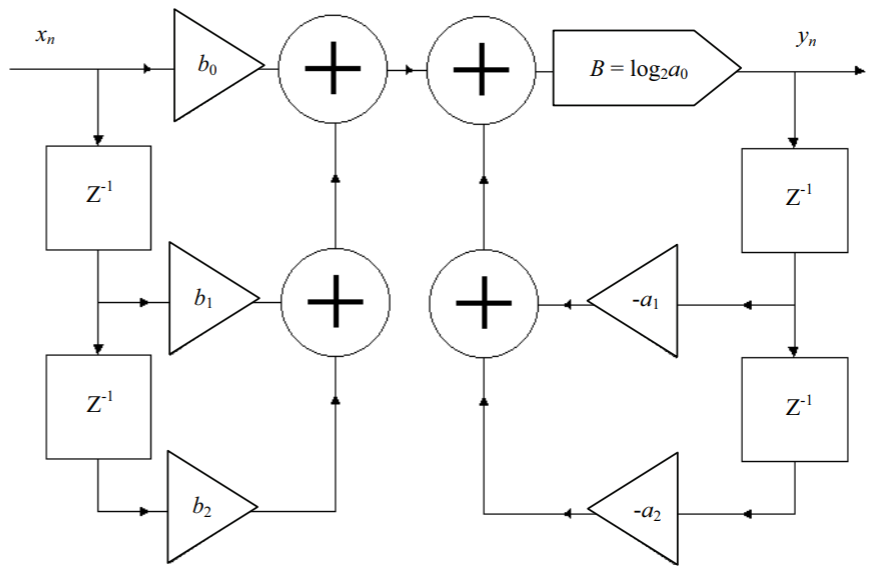
\includegraphics[width=\textwidth]{img/img1}
  \caption{Структура звена рекурсивного ЦНП-фильтра}
  \label{fig:figure1}
\end{figure}

Формально задача машинного синтеза рекурсивного фильтра описывается системой
\begin{gather}
\left\{\begin{aligned}
  &F^{o}\left(\boldsymbol{I X}^{\boldsymbol{o}}\right)=
    \min F(\boldsymbol{I X}),  \quad
      \boldsymbol{I X} \in I^{6 m},\\
  &-2^{R-1} \leq a_{d i} \leq 2^{R-1}-1, \quad \quad d=0,2, \quad i=1,\ldots,m\\
  &a_{0 i} \leq 2^{R-1}-1, \quad d=0,2, \quad \quad i=1,\ldots,m\\
  &a_{0 i} \in\left\{2^{q}\right\}, \quad \quad q=0,\ldots,R-1\\
  &\left(\left|b_{0 i}\right|+\left|b_{1 i}\right|+\left|b_{2 i}\right|+\left|a_{1 i}\right|+\left|a_{2 i}\right|\right)<2^{R-1}, \quad \quad i=1,\ldots,m
\end{aligned}\right.
\end{gather}
где $I^{6m}$ -- целочисленное пространство параметров фильтра, $m$ -- число звеньев второго порядка, $d$ -- индекс коэффициента передаточной функции звена \eqref{eq:iir_cascad}.

Общая экстремальная задача синтеза записана относительно целочисленного пространства $I^{6m}$ параметров (коэффициентов фильтра). Поисковое итеративное решение экстремальной задачи ЦНП в заданном пространстве параметров осуществляет программный алгоритмический комплекс через
модельный блок программы для расчёта текущих функциональных характеристик фильтра. 

Вектор $\boldsymbol{I X}^{\boldsymbol{o}}$, минимизирующий скалярную
целевую функцию $F$, является эффективным решением задачи параметрического синтеза рекурсивного ЦНП-фильтра.

\subsection{Некурсивные фильтры}

В нерекурсивных ЦНП-фильтрах отклик фильтра  вычисляется через прямую линейную свёртку значений входной КИХ-последовательности $x_n$ 
\begin{equation}
  y_{n}=\sum_{k=0}^{N-1} \frac{b_{k}}{a_{0}} \cdot x_{n-k},
\end{equation}
поэтому такие фильтры всегда устойчивы и имеют конечную импульсную характеристику (finite impulse response -- FIR). Входное окно КИХ-фильтра составляет $N$ отсчётов, при этом значение $N$ определяет порядок нерекурсивного фильтра.

Передаточная функция каскадного соединения $m$-звеньев второго порядка нерекурсивного ЦНП-фильтра может быть записана так:
\begin{equation}
  H(z)=\prod_{i=1}^{m} \frac{b_{0 i}+b_{1 i} z^{-1}+b_{2 i} z^{-2}}{a_{0 i}}.
\end{equation}

Уравнение одного звена нерекурсивного фильтра имеет вид:
\begin{equation}
  y_{n}=\frac{b_{0} x_{n}+b_{1} x_{n-1}+b_{2} x_{n-2}}{a_0},
\end{equation}
где коэффициент $a_0$  во всех  $m$  звеньях также принадлежит биномиальному целочисленному ряду $a_{0 i} \in\left\{2^{q}\right\}, q=\overline{0, R-1} \quad i=\overline{1, m}$. На рис. \ref{fig:figure2} приведена типичная структура звеньев нерекурсивного цифрового фильтра.

\begin{figure}[H]
  \centering
  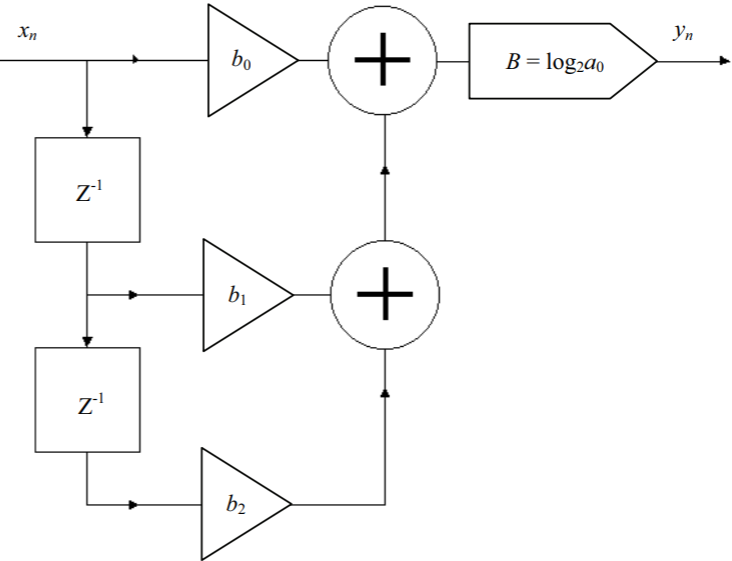
\includegraphics[width=\textwidth]{img/img2}
  \caption{Структура звена нерекурсивного ЦНП-фильтра}
  \label{fig:figure2}
\end{figure}

Постановка задачи целочисленного нелинейного программирования для машинного синтеза нерекурсивного фильтра выглядит следующим образом:

\begin{gather}
\left\{\begin{aligned}
  &F^{o}\left(\boldsymbol{I X}^{\boldsymbol{o}}\right)=
    \min F(\boldsymbol{I X}),  \quad
      \boldsymbol{I X} \in I^{4 m},\\
  &-2^{R-1} \leq b_{d i} \leq 2^{R-1}-1, \quad \quad d=0,2, \quad i=1,\ldots,m\\
  &a_{0 i} \in\left\{2^{q}\right\}, \quad \quad q=0,\ldots,R-1\\
  &\left(\left|b_{0 i}\right|+\left|b_{1 i}\right|+\left|b_{2 i}\right|\right)<2^{R-1}, \quad \quad i=1,\ldots,m
\end{aligned}\right.
\end{gather}
где $I^{4m}$ -- целочисленное пространство параметров фильтра, $m$ - число КИХ-звеньев второго
порядка, $d$ -- индекс коэффициента передаточной функции одного звена КИХ-фильтра, $R$ -- разрядность микропроцессора. 


\section{Лабораторная установка}

Для выполнения лабораторной работы используются три программных модуля: 
\begin{itemize}
  \item программа параметрического синтеза и анализа ЦНП-фильтров,
  \item среда программирования микроконтроллера IAR,
  \item панорамный измеритель частотных характеристик фильтра. 
\end{itemize}
\begin{figure}[H]
  \centering
  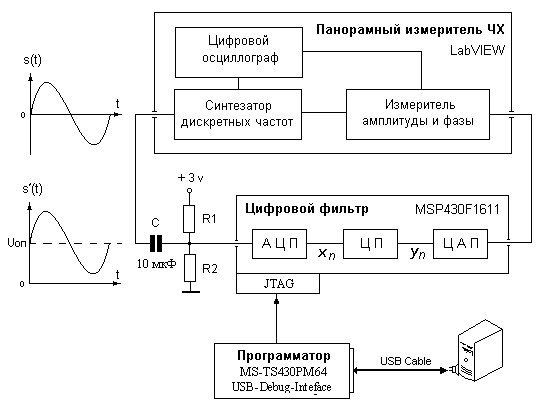
\includegraphics[width=\textwidth]{img/img3}
  \caption{Схема лабораторной установки}
  \label{fig:figure3}
\end{figure}

В лабораторную установку входят отладочная плата MSP-FET430UIF с микроконтроллером MSP430F1611, на котором реализован исследуемый ЦЦФ. Программирование микроконтроллера осуществляется с помощью программатора MSP-TS430PM64 через интерфейс JTAG. 

Измерение частотных характеристик фильтра осуществляется на реальном сигнале с помощью автоматизированной панорамной измерительной системы, разработанной в среде виртуальных приборов LabVIEW. Синтезатор частоты генерирует качественный гармонический сигнал амплитудой 0,5 вольта на дискретных частотах заданного пользователем интервала измерения от частоты $f_{\min}$ до частоты $f_{\max}$ с шагом $f_s$ (все частоты задаются в Гц). Сигнал с синтезатора частоты в положительной полярности подаётся на вход АЦП цифрового фильтра, а выходной сигнал ЦАП – на измеритель амплитуды и фазы. Время генерации входного гармонического сигнала -- 10 периодов на каждой дискретной частоте. Этого вполне достаточно для полного установления колебаний в исследуемой системе. В конце каждого интервала генерации производится измерение амплитуды и фазы выходного сигнала. 
  
Форма входного и выходного сигналов на каждой дискретной частоте отображается на панели цифрового осциллографа, входящего в состав панорамного измерителя частотных характеристик. После завершения измерений в заданном интервале частот производится построение графиков АЧХ и ФЧХ исследуемого фильтра. Эти графики могут быть распечатаны или сохранены в файле средствами LabVIEW.


\subsection{Программа синтеза и анализа цифровых фильтров}
Программа позволяет осуществлять параметрический синтез как рекурсивных (IIR), так и нерекурсивных (FIR) цифровых фильтров различного порядка в широкой области допустимых изменений целочисленных параметров (коэффициентов) фильтра, проводить подробный анализ полученного оптимального решения в частотной области, выводить на печать графики частотных характеристик синтезированного фильтра, а также формировать файл протокола решения текущей задачи синтеза. 
\begin{figure}[h!]
  \centering
  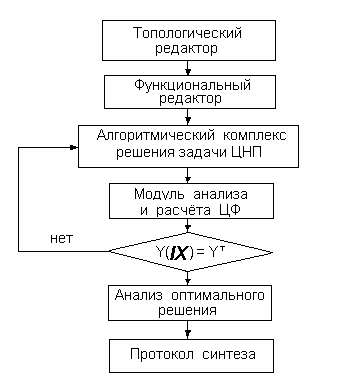
\includegraphics[width=0.6\textwidth]{img/img4}
  \caption{Блок-схема учебной программы синтеза}
  \label{fig:figure1}
\end{figure}
Рассмотрим взаимодействие основных модулей программы в контексте выполнения основных этапов решения конкретной задачи синтеза цифрового фильтра.

\textbf{На первом этапе} формируется типовой топологический файл задания на синтез  name.top, имя которого определяет пользователь. В данных файлах содержится описание структуры синтезируемого фильтра, определяются границы изменения его варьируемых коэффициентов и их начальное значения, указывается порядок и тип синтезируемого фильтра.

\textbf{На  втором этапе} необходимо осуществить ввод требуемых характеристик синтезируемого фильтра и сформировать целевую функцию. Для этого служит графический редактор функциональных характеристик (функциональный редактор), который необходимо вызвать из основного меню программы.

\textbf{На третьем этапе} программный алгоритмический комплекс осуществляет поисковое итеративное решение экстремальной задачи ЦНП-синтеза в заданном пространстве целочисленных варьируемых коэффициентов фильтра, обращаясь к модельному блоку программы для расчёта текущих функциональных характеристик фильтра по заданной его модели. Старт синтеза осуществляется нажатием соответствующей «горячей» кнопкой основного меню программы.

\textbf{На четвёртом этапе} осуществляется подробное исследование найденного эффективного решения задачи ЦНП-синтеза в модуле анализа пакета (кнопка основного меню «Анализ») с построением графиков всех характеристик цифрового фильтра, их распечаткой и формированием стандартного протокола решения задачи синтеза.

\subsection{Микроконтроллер и его программирование}

В данной лабораторной работе изучаются вопросы программной реализации синтезированного целочисленного фильтра на микропроцессорном контроллере, широко используемом в современной радиоэлектронике в качестве встроенного средства контроля, цифровой обработки или управления характеристиками различных объектов или процессов. 

На кристалле такого контроллера, кроме микропроцессора, находятся весь набор необходимых компонентов  вычислительного комплекса, таких как АЦП, системный контроллер, устройства постоянной и перепрограммируемой памяти, аппаратные умножители и сумматоры, ЦАП и др.

Реализация синтезированного ЦНП-фильтра сводится к программированию микроконтроллера, т.е. занесению в ПЗУ найденных целочисленных коэффициентов фильтра и программы их обработки –- расчёта выходного отклика фильтра по его линейно-разностному уравнению  для рекурсивного фильтра либо по прямой свёртке для нерекурсивного.

Программирование микроконтроллера ведётся в среде IAR Emb\-edd\-ed Wo\-rkbe\-nch for MSP430 на языке С++. 
В состав среды программирования входят компилятор, редактор с подсветкой синтаксиса, менеджер проектов, инструментальные средства отладки. Компилятор, входящий в пакет, представляет собой узкоспециализированный компилятор C, который генерирует код на ассемблере TI/IAR MSP430. Загрузка программы в память контроллера осуществляется с помощью встроенного в эту среду FET-Debugger, использующего интерфейс JTAG.
\newpage


\section{Синтез цифровых целочисленных фильтров}
\subsection{FIR-фильтры}
\subsubsection{Гауссов фильтр}
Нормированная резонансная характеристика для гауссовой кривой определяется как
\begin{equation}
  y(\xi)=e^{-\frac{\xi^{2}}{\alpha}},
\end{equation}
где  $\xi=f-f_0$ -- абсолютная расстройка от резонансной частоты, а параметр $\alpha$  определяет нормированную полосу пропускания гауссовой кривой:
\begin{equation}
  \alpha=\frac{\Pi^{2}}{4 \ln \sqrt{2}}
\end{equation}
здесь $\Pi$ -- абсолютная полоса пропускания по уровню 0.7. 
% Выполнение задания в пакете синтеза осуществляется в следующей последовательности.
\subsection{IIR-фильтры}

\section{Реализация IIR-рециркулятора на MSP430}






\addcontentsline{toc}{section}{Заключение}
\section*{Заключение}

В процессе выполнения работы были синтезированы рекурсивные и не рекурсивные модельные  ЦНП – фильтры и фильтры на микроконтроллере, оценены селективные свойства и рекомендуемый рабочий диапазон для данного микроконтроллера, который составил интервал  от 300 Гц до 4000 Гц. Также были реализованы  рекурсивный ЦНП – рециркулятор   и цифровой фильтр нижних частот.

\begin{thebibliography}{}

  \bibitem{met1} Вайнштейн Л.А. Электромагнитные волны. М.: Радио и связь, 1988.

  \bibitem{lit3} Ландау Л.Д., Лифшиц Е.М. Теория поля. М.: Физматлит, 2003.
\end{thebibliography}

\end{document}